%%%%%%%%%%%%%%%%%%%%%%%%%%%%%%%%%%%%%%%%%%%%%%%%%%%%%
\documentclass[apj]{emulateapj}
%\documentclass[preprint2]{aastex61}
%\documentclass[12pt,preprint]{aastex}
\graphicspath{{figures/}}
\DeclareGraphicsExtensions{.jpg,.pdf,.png,.eps,.ps}

\usepackage[table,usenames,dvipsnames]{xcolor}
\usepackage{amsmath}
\usepackage{subfigure}
\usepackage[backref,breaklinks,colorlinks,citecolor=blue]{hyperref}
\usepackage{natbib}
%\usepackage{natbib}
\bibliographystyle{fapj}
\usepackage{graphicx}
\usepackage{multirow}
\usepackage{soul}

%\newcommand{\jcap}{JCAP}

\newcommand{\sqdeg}{deg$^2$ }
\newcommand{\omb}{\ensuremath{\Omega_b h^2}}
\newcommand{\omc}{\ensuremath{\Omega_c h^2}}
\newcommand{\clpp}{\ensuremath{C_{L}^{\phi\phi}}}
\newcommand{\cpmf}{\ensuremath{C_{\ell}^{\rm PMF}}}

\newcommand{\cpmftens}{\ensuremath{C_{\ell}^{\rm PMF,\,tens}}}
\newcommand{\cpmfvec}{\ensuremath{C_{\ell}^{\rm PMF,\,vec}}}
\newcommand{\apmf}{\ensuremath{A_{\rm PMF}}}
\newcommand{\bpmf}{\ensuremath{B_{\rm 1\,Mpc}}}
\newcommand{\alens}{\ensuremath{A_{\rm lens}}}
\newcommand{\lcdm}{\ensuremath{\Lambda}CDM}
\newcommand{\nrun}{\ensuremath{n_{\rm run}}}
\newcommand{\neff}{\ensuremath{N_{\rm eff}}}
\newcommand{\ho}{H\ensuremath{_0}}
\newcommand{\mnu}{\ensuremath{\sum m_\nu}}
\newcommand{\ukarcmin}{\ensuremath{\mu}{\rm K-arcmin}}
\newcommand{\lknee}{\ensuremath{\ell_{\rm knee}}}
\newcommand{\lcut}{\ensuremath{\ell_{\rm min}}}
\newcommand{\fermilat}{\textit{Fermi}-LAT}

\newcommand{\be}{\begin{equation}}
\newcommand{\ee}{\end{equation}}
\newcommand{\planck}{{\sl Planck}}
\newcommand{\wmap}{{\sl WMAP}}
\newcommand{\bicepkeck}{BICEP2/Keck Array}
\newcommand{\sptnew}{SPT-3G }
\newcommand{\pb}{\textsc{Polarbear}}
\newcommand{\simons}{Simons Array}
\newcommand{\sptpol}{SPTpol}
\newcommand{\advactpol}{Adv.~ACTpol }

\newcommand{\tbd}[1]{\textcolor{Red}{{\bf TBD}: #1}}
\newcommand{\gab}[1]{\textcolor{Orchid}{[{\bf GS}: #1]}}
\newcommand{\changed}[1]{\textcolor{Red}{#1}}
\newcommand{\removed}[1]{\textcolor{Red}{}}
\include{number_list}

%

% ref to section \S\ref{sec:label}

%\submitjournal{ApJ}
\def\Melbourne{1}
\def\uci{2}
%%%%%%%%%%%%%%%%%%%%%%%%%%%%%%%%%%%%%%%%%%%%%%%%%%%%%
\begin{document}

\title{Extreme Digitisation For Ground-Based Cosmic Microwave Background Experiments}
\author{L.~Balkenhol\altaffilmark{\Melbourne} and C.~L.~Reichardt\altaffilmark{\Melbourne}}
\altaffiltext{\Melbourne}{School of Physics, University of Melbourne, Parkville, VIC 3010, Australia}
\email{lbalkenhol@student.unimelb.edu.au}

\begin{abstract}

The large size of the time ordered data of cosmic microwave background experiments presents challenges for mission planning and data analysis. These issues are particularly significant for Antarctica- and space-based experiments, which depend on satellite links to transmit data. We explore the viability of reducing the time ordered data to few bit numbers to address these challenges. Unlike lossless compression, few bit digitisation introduces additional noise into the data. We present a set of one, two, and three bit digitisation schemes and measure \changed{the} increase in noise in the cosmic microwave background temperature and polarisation power spectra. The digitisation noise is independent of angular scale and is well-described as a constant percentage of the original detector noise. Three bit digitisation increases the map noise level by $< 2\%$, while reducing the data volume by a factor of \changed{twenty relative to 64}-bit floats. \changed{Comparable gains are seen when extreme digitisation is combined with  
established lossless compression algorithms. Extreme} digitisation is a promising strategy for upcoming experiments.

\end{abstract}

%C: maybe sub techniques:misc for methods: data analysis ? unfortunately no data compression tag
\keywords{cosmic background radiation --- polarization --- techniques: miscellaneous}
\section{Introduction}
\label{sec:intro}

Observations of the cosmic microwave background (CMB) have played a key role in cosmology \citep{penzias1965, smoot1992, bennett2013, sptpol2013, planck2018}. Current ground-based CMB experiments, like \sptnew \citep{benson2014} at the South Pole telescope (SPT) and \advactpol \citep{thornton2016}, at the Atacama cosmology telescope (ACT), target science goals such as the discovery of inflationary gravitational waves, measuring the number of relativistic species, the neutrino mass sum, and mapping the large-scale distribution of matter through gravitational lensing and the Sunyaev-Zeldovich (SZ) effects. Through lensing and the SZ effects the CMB probes structure formation, reionisation, and is a powerful test for dark matter and dark energy models \citep{s4sciencebook, 2018corecos, litebird2016, pixie2011}.

% CITES FOR PARTICLE PHYSICS WITH CMB, ALSO MAYBE SHUFFLE POSITION OF PARTICLE PHYSICS STUFF, KINDA AWKWARD

Over the last two decades, CMB experiments have gone from single detectors to over $10,000$ detectors. The CMB community has developed a variety of compression techniques and computational approaches to handle the increasing volume of data \citep{tristam2007}. These include the compression of time-ordered data (TOD) into maps \citep{tegmark1997}, bandpower estimation \citep{tegmark1998}, and the pseudo-$C_l$ method \citep{brown2005}.

A potential hurdle for experiments at remote locations are the transmission limitations of satellite links. 
Space-based experiments have employed a combination of lossless and lossy compression techniques, including reduced bits in the TOD \citep{gaztanaga1998, maris2003}. 
Antarctica-based experiments that transmit a portion of their results via a satellite link downsample their data to meet telemetry allocations, but have not yet used few bit digitisation of the TOD. 
As we approach the next generation ground-based experiment, CMB-S4 \citep{s4sciencebook}, and the launch of the new space-based missions COrE+ \citep{core2018}, LiteBIRD \citep{litebird2016}, and PIXIE \citep{pixie2011}, we must consider potential transmission bottlenecks carefully. %C: Is there a reference detailing downsampling of SPT data?

In this work we present the method of extreme digitisation, which reduces a many bit (often 32 or 64 bit) signal to a few bits for ground-based experiments. 
We apply extreme digitisation to simulated TOD and detail the resulting effects on temperature and polarisation power spectra. 
We find that an optimal three bit digitisation scheme adds $<2\%$ to the map noise level.

This work is structured as follows. In section \S\ref{sec:dig} we detail the challenges that come with handling large data volumes, introduce the process of extreme digitisation and lay out the framework used to test its performance. 
We present results for white and $1/f$ detector noise in section \S\ref{sec:results}. 
We summarise our findings in \S\ref{sec:conclusions}.
\changed{We report uncertainties based on the symmetric 68\% confidence regions. }

%This work is structured as follows. We detail the arising challenges in handling large TOD in \S\ref{subsec:problem}. We subsequently formulate extreme digitisation in \S\ref{subsec:extremedigitisation} and lay out the framework used to test its performance in \S\ref{subsec:method}. The details of the power spectrum estimation used are laid out in \S\ref{subsec:psestimation}. We continue by presenting the noise induced through the dicitisation process in \S\ref{subsec:additionalnoise} and summarise our findings in \S\ref{sec:conclusions}. 

%CMB is great; One reason is that there is a history of compression and computational techniques that reduce the load of large datasets. ie maps; bandpowers; pseudo-cls.

%satellites have also reduced bits on TOD; ground based haven't had to yet

%however as we discuss building ever larger arrays at remote sites, we are starting to be limited: spt example.

%in this work we present digitisation for ground-based cmb polarisation measurements.
%teaser results


%The outline of this paper is as follows. 
%We present the digisation schemes in \S\ref{sec:dig}, and their performance in \S\ref{sec:results}
%We summarize our findings in \S\ref{sec:conclusions}. 

\section{Digitisation}
\label{sec:dig}

\subsection{The Challenges Of Large Data Sets}
\label{subsec:problem}

%Data influx + Transmission

The science goals of upcoming CMB experiments depend on achieving substantially faster mapping speeds. Given CMB detectors are generally photon noise limited, improving the mapping speed means adding more detectors. As a result the number of detectors (and data volume) of ground-based experiments has followed an exponential trend like Moore's law, doubling approximately every 2 years \citep{s4sciencebook, Abazajian2015}.

The South Pole is one of the best sites for CMB observations on Earth \citep{chamberlin2001, spt2004}. CMB-S4 plans to include several telescopes at the South Pole \citep{s4sciencebook, barron2018}, which will generate a data influx of $\sim\mathcal{O}(10)\mathrm{Tb/d}$. Transferring this data volume via satellite would be expensive. For context, the transmission allocation for a current CMB experiment, SPT-3G, is $150\mathrm{Gb/d}$. The transmission bottleneck could be overcome by recovering the full data on hard drives every summer and transmitting a downsampled version of the data. Downsampling eliminates high frequency information, which makes it unsuitable for science on small angular scales, such as SZ galaxy clusters. The potential delay (i.e. only getting the high frequency data once a year) also introduces risks by delaying when potential faults or issues at high frequency are noticed. One can reduce these issues by running substantial portions of the analysis at the South Pole, but this comes with its own costs and challenges.

% maybe dont include this
%The Planck mission has demonstrated the merits of carrying out CMB observations from space \citep{planck2018}. Upcoming missions aim to exceed the detector count of Planck by at least an order of magnitude \citep{litebird2014, pixie2011, core2018}. Strategies to meet the telemetry specifications of each mission appear to be in development. It is not clear whether the data compression knowledge developed during the Planck mission will guarantee optimal performance for future satellites. Each mission will most likely have to carefully construct a compression algorithm through a combination of lossless and lossy techniques specific to their requirements.

%Planning+Analysis

Beyond transmission challenges, a larger data volume increases the size and cost of disk arrays and makes end-to-end simulations of experiments for the purpose of optimisation on systematics estimation more time consuming. Given the sheer size of upcoming data sets, full end-to-end simulations may prove impractical for CMB-S4 \citep{s4sciencebook}. The exponential growth of CMB data makes timestream level operations, such as noise removal and map making, increasingly time consuming. Few bit digitisation could ameliorate all of these challenges.

%Ground-based observations have to rely on different planning strategies or aim to reduce the size of the TOD in order to maximise the productivity of the design stage. Space-based missions carry out a similar analysis specific to their instruments to heighten their science output.

%what others have done

The Planck mission has already demonstrated the success of extreme digitisation for space-based CMB \changed{experiments} \citep{maris2003}. \cite{jenet1998} explored the application of few bit digitisation to radio pulsar timing measurements. Recently Clearwater et al. (private communication) have demonstrated the advantages of using one and two bit data when searching for continuous gravitational waves using the Laser Interferometer Gravitational-Wave Observatory (LIGO).


\subsection{Extreme Digitisation}
\label{subsec:extremedigitisation}

The optimal digitisation scheme to minimise distortion for a fixed number of bits depends on the details of the input signal. 
In most cases this optimisation is neglected, since the distortions become vanishingly small as the number of bits increases. However, optimal schemes are critical to the success of extreme (few bit) digitisation. We review the key aspects of designing digitisation schemes as established by \cite{max1960} below.

Digitisation discretises an input signal by sorting it into $N$ ranges, such that an input between $x_i$ and $x_{i+1}$ produces an output value $y_i$. The set of parameters $N, x_i, y_i$ fully specify a digitisation scheme. Conventionally one chooses $x_{1} = -\infty$ and $x_{N+1} = \infty$, i.e. values beyond some threshold saturate and yield identical output. In order to quantify the performance of a given digitisation scheme we define the distortion as
\begin{equation}\label{eq:distdef}
D = \left\langle  \left( s - \hat{s} \right)^2 \right\rangle,
\end{equation}
where $s$ is the input and $\hat{s}$ the output signal. For a stochastic input signal we can calculate an amplitude probability distribution $p(x)$. \changed{This allows us to re-express the distortion as a sum over the digitisation levels:}

\begin{equation} \label{eq:dist}
D = \sum_{i = 1}^N \int_{x_i}^{x_{i+1}} \left(x-y_i\right)^2 p(x) dx.
\end{equation}

Since we wish to minimise the distortion, we set \changed{its derivatives} with respect to $x_i$ and $y_i$ to zero. Starting with $x_i$ we obtain

\begin{equation} \label{eq:distderiv1}
\frac{\partial D}{\partial x_i} = \left(x_i-y_{i-1}\right)^2 p(x_i) - \left(x_i - y_i\right)^2 p(x_i) = 0.
\end{equation}

\begin{equation} \label{eq:digitequalspacecondition}
x_i = \frac{y_i+y_{i+1}}{2},
\end{equation}
which informs us that the threshold levels should lie midway between their adjacent output levels. Setting the derivative of equation \ref{eq:dist} with respect to $y_i$  to zero gives the additional condition
\begin{equation} \label{eq:distderiv2}
\frac{\partial D}{\partial y_i} = -2 \int_{x_i}^{x_{i+1}} \left( x-y_i \right) p(x) dx = 0.
\end{equation}

\begin{equation} \label{eq:digitareacondition}
\int_{x_i}^{x_{i+1}} \left( x-y_i \right) p(x) dx = 0.
\end{equation}
This \changed{condition} implies that we should choose $y_i$, such that it halves the area underneath $p(x)$ in the interval from $x_i$ to $x_{i+1}$.

To progress further, we must consider the probability distribution $p(x)$ of the input signal. 
\changed{In this work, we are interested in the compression of the TOD from each detector of a ground-based CMB experiment. 
Thus we can safely assume that the input signal is in the low signal-to-noise regime. 
Furthermore, we take the simplest noise profile: Gaussian, white detector noise\footnote{\changed{As discussed in the appendix, this treatment also applies to more realistic noise profiles, because the large number of points lying in each map pixel allows the application of the central limit theorem.}}. 
Together these assumptions imply that the input, $x$, is normally distributed, with} $p(x) = (1/\sqrt{2\pi\sigma^2}) e^{-x^2/2\sigma^2}$. 

\changed{\citet{max1960} solved Equations \ref{eq:digitequalspacecondition} and \ref{eq:digitareacondition} for 1-, 2- and 3-bit digitisation for this choice of probability distribution, $p(x)$. 
We quote their results below and refer the reader to the aforementioned work for the derivation.  
As one would expect given the symmetry in $p(x)$, the 1-bit (N=2 output levels) case is simply:
\begin{equation} \label{eq:1bit}
\hat{s}_1(t) = \left\{ \begin{array}{lr}
1, & s(t) > 0\\
-1, & s(t) \leq 0
\end{array} \right. \hspace{0.5cm}.  \end{equation}
Essentially, the optimal 1-bit digitisation scheme applies the sign function to the TOD. 
}

\changed{
For two bit digitisation, we can encode $N=4$ output levels. The optimal set of thresholds and digitisation levels is given by the four-level function:}
\begin{equation}  \label{eq:2bit}
\hat{s}_2(t) = \left\{ \begin{array}{rl}
1.51 \sigma, & s(t) \geq 0.98 \sigma\\
0.45 \sigma, & 0 \leq s(t) < 0.98 \sigma\\
-0.45 \sigma, & -0.98 \sigma \leq s(t) < 0\\
-1.51 \sigma, & -0.98 \sigma < s(t)\\
\end{array} \right. \hspace{0.5cm}.  \end{equation}
%C: should i round to equal significant figures here? Unfortunately these are the exact values that i used...

\changed{Finally, with 3 bits we may specify $N=8$ output levels. The optimal three bit digitisation is described by the eight-level function:}
\begin{equation}  \label{eq:3bit}
\hat{s}_3(t) = \left\{ \begin{array}{rl}
2.15 \sigma, & s(t) \geq 1.75 \sigma\\
1.34 \sigma, & 1.05 \sigma \leq s(t) < 1.75 \sigma\\
0.76 \sigma, & 0.50 \sigma \leq s(t) < 1.05 \sigma\\
0.25 \sigma, & 0 \leq s(t) < 0.50 \sigma\\
-0.25 \sigma, & -0.50 \sigma \leq s(t) < 0\\
-0.76 \sigma, & -1.05 \sigma \leq s(t) < -0.50 \sigma\\
-1.34 \sigma, & -1.75 \sigma \leq s(t) < -1.05 \sigma\\
-2.15 \sigma, & -1.75 \sigma < s(t)\\
\end{array} \right. \hspace{0.5cm}.  \end{equation}

\changed{The digitisation schemes above are designed to minimise the distortion of the TOD as defined in Equation \ref{eq:distdef}. This does not ensure that the digitised output has the same signal power as the input. However, the output of the schemes given above can be rescaled by a constant to achieve power conservation. This is demonstrated in the appendix, where we also derive an analytical expression for the normalisation constant. We use this analytical rescaling for all results in this work.
}

%This is not particularly important, since most CMB experiments determine the absolute calibration from their maps. However, 

%However, it is worth noting that one can rescale the schemes laid out by \cite{max1960} to preserve power, which is demonstrated in the appendix.

%Completely different digitisation schemes can be thought of, which would for example reference the most drastic outlier in the data set, or seek to place equal numbers of points into each digitisation level. However, given the assumptions made the schemes derived above minimise the distortion metric defined. Additionally, they are simple enough to be easily implemented computationally. We consider how to design digitisation schemes that preserve the power of the TOD and how to adjust a given digitisation scheme to ensure power conservation in the appendix.

\subsection{From Time Ordered Data To Maps}
\label{subsec:method}

To investigate the performance of the derived digitisation schemes, we simulate timestream level scans over a single CMB realisation. We add detector noise and apply the digitisation schemes above to the simulated I, Q, and U TOD. We also retain the original 64 bit TOD to construct control maps. The different timestreams are binned into HEALPix \citep{healpix}\footnote{Available at \url{http://healpix.sourceforge.net/}.} maps with resolution $\mathrm{NSIDE} = 4096$ for a T, E, and B power spectrum analysis.

% We obtain control maps that use 64 bit TOD and maps that have undergone one, two, and three bit digitisation of the TOD. We calculate the temperature and polarisation power spectra of each map and determine the noise level.
%C: Do I need to mention that we assume to have an infinitely fast spinning plate?

We use the healpy Python package to generate a single CMB realisation for the best-fit Planck 2015 cosmology. Specifically, the key cosmological parameters are $H_0 = 67.8 \mathrm{km \> s^{-1} Mpc^{-1}}$, $\Omega_{\mathrm{m}} = 0.308 $, $n_{\mathrm{s}} = 0.968$, and $\tau = 0.066$ \citep{planck2016}.

%C: Do I need to comment on the fact that this reflects no particular frequency channel, but the results come from a combination of all observed channels?

We simulate observing a $600 \> \mathrm{ deg^2}$ patch of the sky with a single detector. The detector noise level for temperature is $500 \mathrm{\mu K \sqrt{s}}$ and for polarisation observations $\sqrt{2} \hspace{0.7ex} 500 \mathrm{\mu K \sqrt{s}}$, i.e. the corresponding photon noise limit. Constant elevation scans (CES) are performed beginning at right ascension (RA) and declination (DEC) $(0^\circ, 0^\circ)$. After covering $24^\circ30'$ along RA the detector is reset to a RA of $0^\circ$ and an offset in DEC corresponding to the pixel size. Through repetition of CES with constant steps in DEC the survey patch is covered. This imitates the scan strategy of the SPT \citep{schaffer2011}. The entire scan strategy is repeated $100$ times with offsets in the starting RA and DEC up to the size of one pixel, ensuring that pixels are sampled uniformly.

We create naive I,Q, and U maps from the simulated I, Q, and U TOD, i.e. the value of a map pixel is the average of all TOD samples lying within that pixel. We create four maps: one using the original 64 bit TOD and one for each of the digitisation schemes. We save the ouput maps at $800$, $8,000$, $80,000$, $1,024,000$, $10,240,000$ and $102,400,000$ hits per pixel.

%The detector is read out at $200\mathrm{Hz}$ and the on sky speed is adjusted between simulation to produce the desired number of hits per map pixel. The detector noise level for temperature is $500 \mathrm{\mu K \sqrt{s}}$ and for polarisation observations $\sqrt{2} \hspace{0.7ex} 500 \mathrm{\mu K \sqrt{s}}$, i.e. the corresponding photon noise limit.

%During a CES the pixels being targeted are determined. The corresponding values of the input maps are accessed and added to detector noise realisations of the same length as the number of hits falling into each pixel. This is done for I, Q, and U maps, producing three timestreams. A 64 bit copy of the TOD is processed separately and the above digitisation schemes are applied. The four resulting sets of observation data are compressed into maps by averaging all hits falling into the same pixel. This produces 24 CMB maps in total: three control maps and nine maps with three each obtained from the different digitisation schemes. Additionally we keep hold of the hitmap.

%This simulation is implemented in Python. We use parallelisation to navigate memory requirements and reach the depth of observation desired. Artificial observations with $800$, $8,000$, $80,000$, $1,024,000$, $10,240,000$ and $102,400,000$ hits per map pixel are carried out.

%To do so we perform constant elevation scans (CES), equally spaced in declination (DEC). We repeat the observation strategy $100$ times with a slight offset in right ascension (RA) and DEC each time, such that each pixel is sampled approximately uniformly. The detector is read out at $200 \mathrm{Hz}$. The speed at which we sweep across the survey area is adjusted to produce a desired number of hits per pixel in the output maps.

%While performing each CES the pixels being targeted are determined. The corresponding values from the template maps are accessed and added to detector noise realisations. For temperature observations we assume the detector noise level to be $500 \mathrm{\mu K \sqrt{s}}$ and for polarisation observations $\sqrt{2} \hspace{0.7ex} 500 \mathrm{\mu K \sqrt{s}}$, i.e. the corresponding photon noise limit.

%Having constructed I,Q and U TOD we apply the digitisation schemes derived above. We compress the timestreams into maps by averaging all hits falling into the same pixel. This produces 24 CMB maps in total: three control maps and nine maps with three each obtained from the different digitisation schemes. We simulate observations with $800$, $8,000$, $80,000$, $1,024,000$, $10,240,000$ and $102,400,000$ hits per map pixel.

%It is often commonplace to fit a polynomial to the TOD, a series of sines and cosines, subtract local averages or do a combination of these techniques \citep[e.g.][, planck?]{chown2018} to reduce $1/f$ noise. We do not employ any of these filtering mechanisms. A thorough application of such noise removal techniques would lead to similar results as the white noise case.

% LINK TO GITHUB WITH CODE HERE

%The calculation outlined above has considerable computational requirements if we want to reach up to $\sim 10^8$ hits per pixel. This calculation was made possible through use of the NERSC facilities.

\subsection{Power Spectrum Estimation}
\label{subsec:psestimation}

To minimise boundary effects in the subsequent analysis we apodise the observed patch using a cosine mask. For the case of white detector noise we use PolSpice \citep{polspice} to compute $\mathrm{TT}$, $\mathrm{EE}$ and $\mathrm{BB}$ power spectra from output maps. 

For the later considered case of anisotropic noise, we use healpy to calculate the spherical harmonic coefficients $a\ell m$. Since the scan strategy of the simulated observations is similar to the SPT's, smaller values of $m$ correspond to larger angular features along the scan direction \citep{chown2018}. Because of the anisotropic nature of the noise, equally weighting all modes leads to inaccurate power spectra. As a first order approximation to optimal weighting we discount the lowest modes in scan direction.

We rebin the calculated power spectra as mentioned \changed{when applicable} and assign Fisher matrix error bars \citep{tegmarkdesignersguide1997}.

As seen in Figure \ref{fig:psrecover} (appendix) all spectra of extremely digitised data recover the input to a satisfying degree. Differences between few bit and the input power spectra are due to observing a single CMB realisation and residual boundary effects.

\section{Results}
\label{sec:results}

\subsection{White Noise}
\label{subsec:whitenoise}

We analyse the results of the simulated observations to quantify the distortion digitisation causes in the power spectra and investigate whether the additional noise has any angular scale dependence.

%This will show us whether extreme digitisation is viable for the observations targeted by CMBS-4.
We infer the fractional increase of the original map noise level, $\Delta \sigma / \sigma$, to quantify the distortion caused by extreme digitisation. We calculate $\Delta \sigma / \sigma$ from the noise dominated angular scales in the power spectra via

\begin{equation}
\frac{\Delta \sigma}{\sigma} = \sqrt{1 + \frac{C_\ell^\mathrm{X}}{C_\ell^{\mathrm{N}}}} - 1,
\end{equation}

where $C_\ell^{\mathrm{N}}$ and $C_\ell^\mathrm{X}$ are the detector noise level and the additional digitisation noise respectively. Before calculating $C_\ell^\mathrm{X}/C_\ell^\mathrm{N}$ we rebin the power spectra to $\Delta \ell \approx 100$. This ensures that points in the noise tail are independent, allowing us to extract an uncertainty for $\Delta \sigma / \sigma$.

%We formulate

%\begin{equation} \label{eq:extramapnoise}
%\frac{\Delta \sigma}{\sigma} = \frac{\sigma_{\mathrm{map}}^{\mathrm{D}}-\sigma_{\mathrm{map}}^{\mathrm{C}}}{\sigma_{\mathrm{map}}^{\mathrm{C}}},
%\end{equation}

%where $\sigma_{\mathrm{map}}^{\mathrm{C}}$ and $\sigma_{\mathrm{map}}^{\mathrm{D}}$ are the map noise levels of control observations and simulations using few bit TOD respectively. In the noise dominated regime

%\begin{equation} C_{\ell}^\mathrm{D} = C_\ell^\mathrm{N} + C_\ell^\mathrm{X}, \end{equation}

%where $C_{\ell}^\mathrm{D}$, $ C_\ell^\mathrm{N}$, and $C_\ell^\mathrm{X}$ are the power spectra of few bit data, the detector noise level, and the additional noise due to digitisation respectively. We progress equation \ref{eq:extramapnoise} to

%\begin{equation}\frac{\Delta \sigma}{\sigma} = \sqrt{\frac{C_l^\mathrm{D}}{C_l^{\mathrm{N}}}} - 1 = \sqrt{1 + \frac{C_\ell^\mathrm{X}}{C_\ell^{\mathrm{N}}}} - 1. \end{equation}

The deduced additional noise for one, two, and three bit digitisation is shown in Table \ref{tab:extranoisewhite} in the appendix. 
We see that 3 bit digitisation performs best, followed by two bit and one bit. 
This is expected, since more bits allow a more faithful representation of the input signal. 
We observe that the fractional increase, $\Delta \sigma / \sigma$, is independent of the hits per pixel in the maps and that the compression performs as well for polarisation as is does for temperature data. \changed{Finally, it is striking how little noise is added. 
On average one-bit digitisation leads to a $(25.13\pm 0.94)\%$ increase in the map noise level, two-bit yields a $(6.40\pm0.41)\%$ increase and three-bit adds only $(1.76\pm0.22)\%$. 
This is impressive, given that all schemes considered reduce the TOD volume by at least an order of magnitude.}

To investigate whether the noise added through digitisation has any angular scale dependence, we subtract the input map from simulated observations. The power in the difference map is plotted in Figure \ref{fig:diffpswn}. There is no sign of any angular scale dependence.

% This is in agreement with (planck website) but does not match the results of (planck short paper). This is likely due to the intricities of the planck compression scheme differing to what is considered here. A full comparison is difficult in the absense of a detailed description of the simulations carried out in either paper.

\begin{figure}[htb]\centering
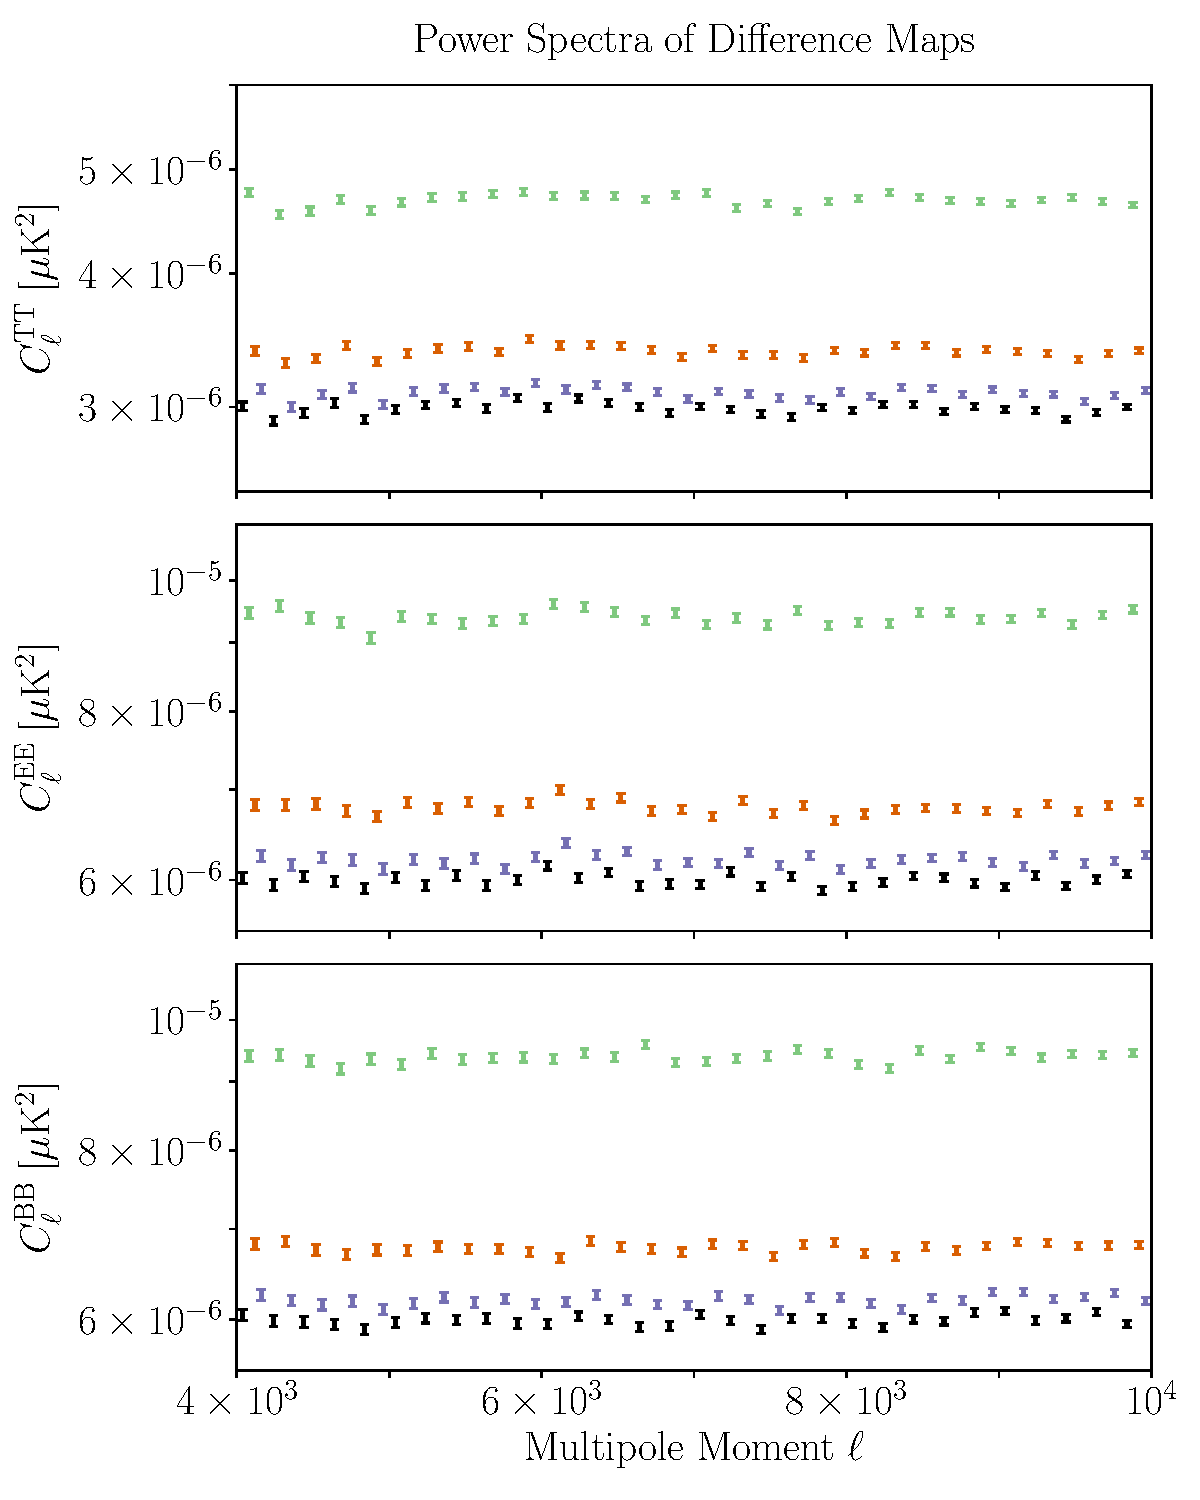
\includegraphics[width=0.5\textwidth,clip]{diffwn.pdf}
  \caption[Current ]{
  \changed{TT, EE, and BB power spectra (upper, middle and lowest panel respectively) of difference maps for one-bit (green marker, high), two-bit (orange marker, medium), and three-bit digitisation (violet marker, low). The control case using 64-bit TOD is also shown (black marker). All power spectra are rebined to $\Delta \ell = 200$. The vertical axes are logarithmic. The noise increase due to digitisation appears to be independent of angular scale. This plot shows results for a simulation with $1,024,000$ hits per map pixel using Gaussian white detector noise.}
\label{fig:diffpswn}
}
\end{figure}

\subsection{1/f Noise}
\label{subsec:oofnoise}

\changed{While digitisation clearly works extremely well for white noise, real experiments face several sources of low-frequency noise. 
High on the list for ground-based experiments is atmospheric noise. 
For typical observing conditions in Antarctica, the atmosphere turbulence is well-described by Kolmogorov turbulence in the thin-sheet regime \citep{bussmann2005}. 
In this regime, we can describe fluctuations with the noise profile \citep{lay2000}:}

\changed{
\begin{equation} \label{eq:1/fnoiseform}
\left| N_{1/f}(\ell_{\mathrm{scan}}) \right|^2 = \left| N_{\mathrm{white}} \right|^2 \left[ 1 + \left( \frac{\ell_{\mathrm{scan}}}{\ell_0} \right)^{-3/2} \right]^2,
\end{equation}
}

%  exp\left[ -\left( \frac{\lcut}{\ell} \right)^{12} \right]

where $N_{\mathrm{white}}$ denotes white detector noise. In this expression \changed{$\ell_{\mathrm{scan}}$} describes the multipole moment of angular features of corresponding size along the scan direction. The scale at which such modes are amplified appreciably by the second term in equation \ref{eq:1/fnoiseform} is set by \changed{$\ell_0$}. \changed{The exponent of $\ell_{\mathrm{scan}}/\ell_0$ is chosen to model observation at a constant, moderate elevation \citep{lay1997}. In line with the observed noise profile of the SPT we choose $\ell_0 = 1000$ for temperature and $\ell_0 = 0$ for polarisation; this means that power is doubled at $\lknee \approx 1800$ and $\lknee \approx 90$ for temperature and polarisation, respectively \citep{henning2018}.} In practice CMB experiments suppress power in the lowest modes through a range of techniques, including fitting polynomials, sines, and cosines to the TOD. We simulate successful removal of these modes by applying a high pass filter to the noise, such that

\changed{
\begin{equation} \label{eq:1/fnoiseformfinal}
\left| N (\ell_{\mathrm{scan}}) \right|^2 = \left| N_{1/f}(\ell_{\mathrm{scan}}) \right|^2 \exp\left[ -2\left( \frac{\lcut}{\ell_{\mathrm{scan}}} \right)^{6} \right],
\end{equation}
}

with $\lcut = 336.3$ for temperature and $\lcut = 16.8$ for polarisation.

We use the same digitisation schemes as for white noise, but \changed{replace} the parameter $\sigma$ in equations \ref{eq:1bit}, \ref{eq:2bit} and \ref{eq:3bit} by considering Parseval's theorem on the above noise profile. The appropriate value is obtained by \changed{numerically} evaluating the integral

\begin{equation} \label{eq:psvl1/f}
\sigma^2 = \int_0^\infty \left| N(\ell) \right|^2 d\ell.
\end{equation}

After modifying the digitisation schemes derived in subsection \S\ref{subsec:extremedigitisation} accordingly, we carry out the same simulations as described in subsection \S\ref{subsec:method} with the noise profile given in equation \ref{eq:1/fnoiseformfinal}. We save the output maps at $8,000$, $102,400$ and $1,024,000$ hits per pixel. The analysis procedure of subsection \S\ref{subsec:whitenoise} is used to characterise the digitisation noise.

% ------------ maybe dont include this ------------
%\changed{Even though the noise profile given in Equation \ref{eq:1/fnoiseformfinal} is anisotropic in Fourier space, the same is not true in real space. In fact, projecting the chosen noise profile onto the sky using our scan strategy we expect the same noise level in each map pixel. Normalisation of the digitised output by a constant is therefore still appropriate. As explained in Section \ref{sec:digitconspow}, the central limit theorem ensures that the noise amplitude probability distribution in each pixel is Gaussian; using the normalisation constant derived in Section \ref{sec:digitconspow} is still appropriate.}

We recover similar results to the white noise case, with three bit digitisation performing the best, followed by two bit, and one bit. Table \ref{tab:extranoiseoof} in the appendix displays the fractional increase to the detector noise level due to digitisation, $\Delta \sigma / \sigma$. While polarisation observations seem to incur a slightly higher noise penalty compared to temperature, deviations do not exceed $3\sigma$. \changed{On average one-bit digitisation leads to a $(24.4\pm 1.4)\%$ increase in the map noise level, two-bit adds $(6.21\pm0.50)\%$, and three-bit yields an increase of only $(1.71\pm0.21)\%$. 
The fractional added noise from few-bit digitisation is consistent with being identical for the white noise and realistic noise profiles.}



%\changed{Performing a $t$-test for independent variables, we find that for a given digitisation scheme it is unlikely that the noise increase variates for Gaussian white and low-frequency detector noise are drawn from different underlying distributions (p-values: 0.19, 0.34, and 0.57 for one, two, and three bit, respectively). This result reflects the work of the central limit theorem.}

% find a different home for this
%Extreme digitisation is a viable lossy compression technique when dealing with low signal to noise, large data sets. A signal that varies slowly with respect to the sampling rate can be reconstructed well. A small signal will also prevent saturation of the output, i.e. the inability of the digitised output to represent numbers larger than $y_N N_{\mathrm{hit}}$ or smaller than $y_1 N_{\mathrm{hit}}$, where $N_{\mathrm{hit}}$ is the number of data points in an interval. These conditions are satisfied by CMB data and our findings reflect this.

\subsection{\changed{Interaction with Existing Compression Techniques}}

\changed{Current ground-based CMB experiments already employ 
 lossless and lossy compression techniques to manage their transmission bottlenecks. To test whether few-bit digitisation is competitive to existing lossy compression techniques, it is necessary to see if it still provides a substantial reduction in data volume if used in conjunction with lossless compression algorithms.}

\changed{We focus on lossless compression via the Lempel-Ziv-Markoc chain algorithm (LZMA), which is used by the Background Imaging of Cosmic Extragalactic Polarization (BICEP) experiment, and the free lossless audio codec (FLAC), which the SPT and POLARBEAR experiments employ (private communication). We examine the compression of a single CES of our simulation, consisting of ca. $10^7$ data points, by applying LZMA and FLAC separately to four timestreams: the original 64-bit TOD, and copies that have undergone 1-, 2-, and 3-bit digitisation.}

\changed{We find that even though the data reduction power of few-bit digitisation is decreased when used in conjunction with lossless compression algorithms, substantial savings are still achieved. Applying few-bit digitisation to the TOD prior to compression with FLAC reduces the final file size by a factor $5.89$ compared to the FLAC compressed 64-bit data. This is the same for all digitisation schemes considered. Working with LZMA, the data volume of the TOD can be reduced with respect to compressed 64-bit data by factors of $17.34$, $26.23$, and $44.48$ for 3-, 2-, and 1-bit digitisation, respectively. Few-bit digitisation still achieves considerable data reduction if used together with established lossless compression algorithms.}

\section{Conclusion}
\label{sec:conclusions}

In this work we have conducted an investigation of extreme digitisation as a technique in combating the challenges of large data volumes for ground-based CMB experiments. In particular the reduction of TOD volume by an order of magnitude decreases the transmission requirements from remote locations. The reduction may also streamline the analysis and simulation of TOD.

We present a set of one, two, and three bit digitisation schemes. For white and $1/f$ detector noise alike, we find that optimal three bit digitisation adds as little as $<2\%$ to the map noise level. This is true for temperature and polarisation observations. No change in the results is observed for maps \changed{with different numbers of} hits per pixel and no angular scale dependence was observed in the added noise. \changed{Combining few-bit digitisation with currently used lossless compression codecs reduces its compression power only slightly. Applying three-bit digitisation to TOD prior to lossless compression via FLAC or LZMA reduces the data volume by a further factor of $5.89$ or $17.34$, respectively.}

Given that the digitisation noise remains low at small angular scales, cluster finding algorithms may perform well on few bit TOD. Investigating this will also help determine the higher order statistical moments, i.e. skewness and kurtosis, of the digitisation noise.

\acknowledgments % thank patrick for discussion/starting point? Andrew?

% Melbourne CMB group, funding, NERSC.

We are grateful for insightful discussions about the prospects of extreme digitisation for CMB experiments with Andrew Melatos and Patrick Clearwater.
We thank the \changed{referee as well as Nikhel Gupta, Srinivasan Raghunathan, Federico Bianchini, Andrew Melatos, and Patrick Clearwater for valuable feedback on the manuscript.}
We acknowledge support from an Australian Research Council Future Fellowship (FT150100074), and also from the University of Melbourne. 
This research used resources of the National Energy Research Scientific Computing Center, which is supported by the Office of Science of the U.S. Department of Energy under Contract No. DE-AC02-05CH11231. 
We acknowledge the use of the Legacy Archive for Microwave Background Data Analysis (LAMBDA). Support for LAMBDA is provided by the NASA Office of Space Science.

% all code stuff

This research made use of the NumPy \citep{numpy}, SciPy \citep{scipy}, Matplotlib \citep{matplotlib}, and Astropy \citep{astropy} packages.

\newpage

% APPENDIX
\appendix

\begin{figure*}[h!t]\centering
\vspace{-1.5cm}
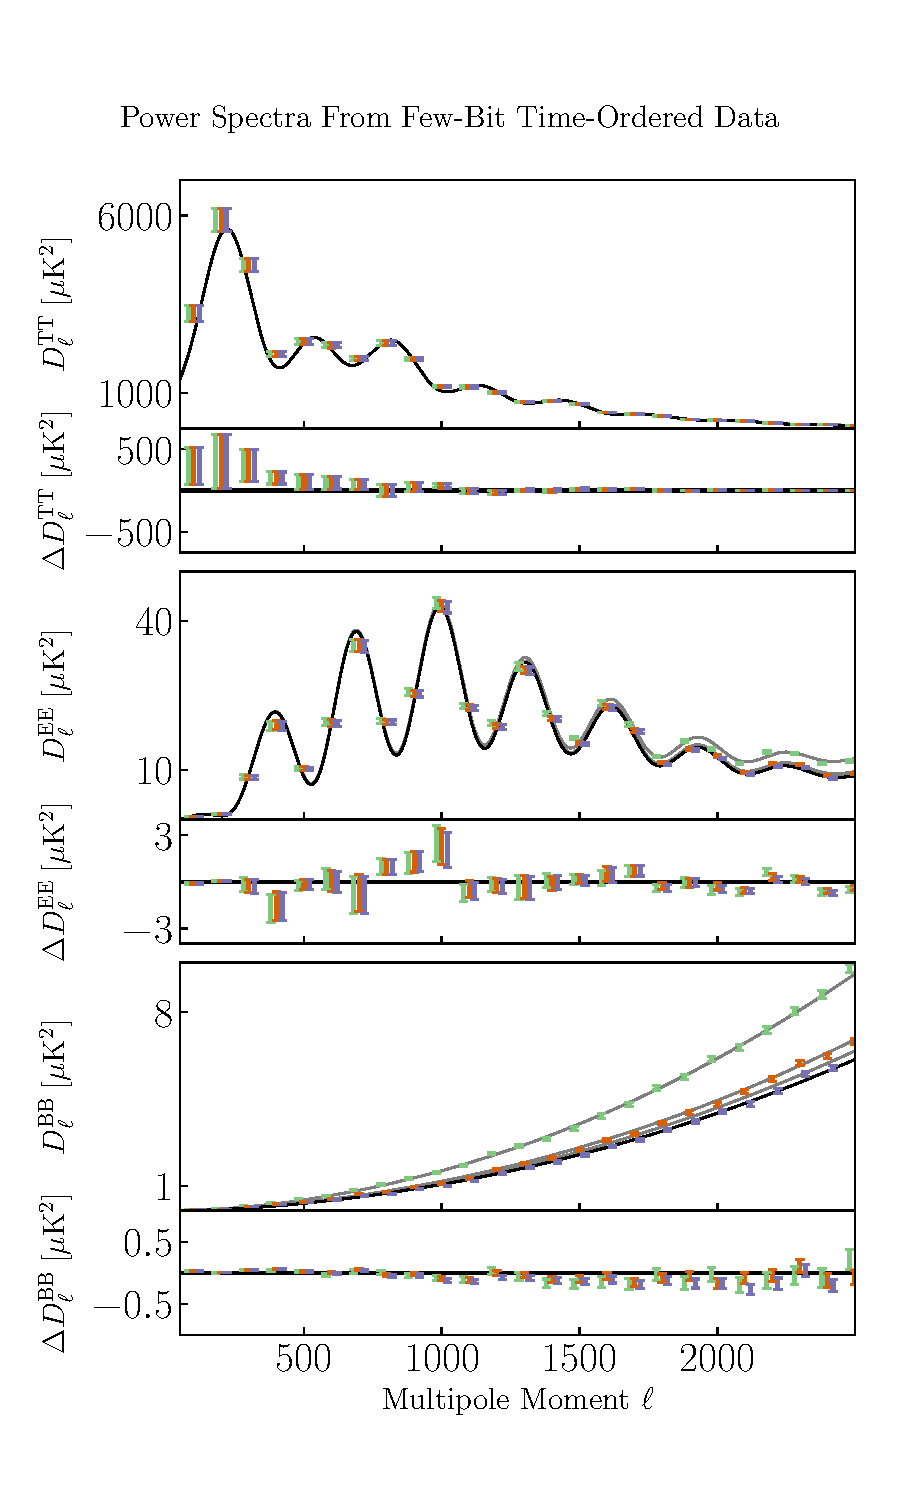
\includegraphics[width=0.8\textwidth,clip]{psrecovery.pdf}
  \caption[Current ]{
  \changed{(FIGURE HAS BEEN CHANGED) Input power spectra used to generate the CMB template map plus detector noise level (black line) and digitisation noise (grey line); power spectra using three- (violet marker, right), two- (orange marker, middle), and one-bit (green marker, left) TOD. Power spectra are rescaled to $D_\ell = \ell (\ell+1) C_\ell /2\pi$ and bined to $\Delta \ell = 100$. Main panels show the TT (top), EE (middle), and BB (bottom) power spectra; accompanying panels show the difference between the input plus noise curves and the power spectra recovered from few-bit TOD. Spectra constructed from few-bit TOD recover the input well. This plot shows results for a simulation with $1,024,000$ hits per map pixel using Gaussian white detector noise.}
\label{fig:psrecover}
}
\end{figure*}

% result tables
\subsection{Digitisation Noise Levels}
\label{subsec:appendixnoisetables}

\def\arraystretch{1.3}
\begin{table*}[tbh]
\begin{center}
\caption{\label{tab:extranoisewhite} \changed{Fractional Noise Increase Due To Digitisation - Gaussian White Detector Noise}}
\small
\begin{tabular}{c c c c c}
Hits Per Pixel & Channel & 1 Bit & 2 Bit & 3 Bit \\
\hline
\hline
\multirow{3}{*}{800}  & TT  & $ 0.252 \pm 0.0091 $  & $ 0.0639 \pm 0.0034 $  & $ 0.0173 \pm 0.0021 $ \\
& EE  & $ 0.253 \pm 0.012 $  & $ 0.0640 \pm 0.0047 $  & $ 0.0175 \pm 0.0041 $ \\
& BB  & $ 0.254 \pm 0.011 $  & $ 0.0652 \pm 0.0054 $  & $ 0.0180 \pm 0.0039 $ \\
\hline
\multirow{3}{*}{8,000}  & TT  & $ 0.2521 \pm 0.0076 $  & $ 0.0641 \pm 0.0034 $  & $ 0.0174 \pm 0.0017 $ \\
& EE  & $ 0.2519 \pm 0.0074 $  & $ 0.0636 \pm 0.0040 $  & $ 0.0173 \pm 0.0022 $ \\
& BB  & $ 0.252 \pm 0.018 $  & $ 0.0634 \pm 0.0089 $  & $ 0.0176 \pm 0.0036 $ \\
\hline
\multirow{3}{*}{80,000}  & TT  & $ 0.2526 \pm 0.0080 $  & $ 0.0645 \pm 0.0040 $  & $ 0.0181 \pm 0.0016 $ \\
& EE  & $ 0.2506 \pm 0.0093 $  & $ 0.0641 \pm 0.0042 $  & $ 0.0177 \pm 0.0019 $ \\
& BB  & $ 0.250 \pm 0.012 $  & $ 0.0636 \pm 0.0065 $  & $ 0.0179 \pm 0.0032 $ \\
\hline
\multirow{3}{*}{1,024,000}  & TT  & $ 0.2501 \pm 0.0090 $  & $ 0.0633 \pm 0.0031 $  & $ 0.0173 \pm 0.0016 $ \\
& EE  & $ 0.2518 \pm 0.0080 $  & $ 0.0646 \pm 0.0033 $  & $ 0.0179 \pm 0.0018 $ \\
& BB  & $ 0.2520 \pm 0.0082 $  & $ 0.0639 \pm 0.0037 $  & $ 0.0173 \pm 0.0021 $ \\
\hline
\multirow{3}{*}{10,240,000}  & TT  & $ 0.2480 \pm 0.0078 $  & $ 0.0630 \pm 0.0038 $  & $ 0.0175 \pm 0.0018 $ \\
& EE  & $ 0.2526 \pm 0.0077 $  & $ 0.0647 \pm 0.0033 $  & $ 0.0183 \pm 0.0018 $ \\
& BB  & $ 0.252 \pm 0.010 $  & $ 0.0642 \pm 0.0042 $  & $ 0.0177 \pm 0.0020 $ \\
\hline
\multirow{3}{*}{102,400,000}  & TT  & $ 0.2465 \pm 0.0049 $  & $ 0.0629 \pm 0.0019 $  & $ 0.0170 \pm 0.0010 $ \\
& EE  & $ 0.2511 \pm 0.0078 $  & $ 0.0644 \pm 0.0035 $  & $ 0.0175 \pm 0.0018 $ \\
& BB  & $ 0.2523 \pm 0.0086 $  & $ 0.0640 \pm 0.0031 $  & $ 0.0179 \pm 0.0017 $ \\
\hline
\multirow{3}{*}{Average}  & TT  & $ 0.2502 \pm 0.0017 $  & $ 0.0636 \pm 0.0017 $  & $ 0.0175 \pm 0.0017 $ \\
 & EE  & $ 0.2518 \pm 0.0023 $  & $ 0.0643 \pm 0.0023 $  & $ 0.0177 \pm 0.0023 $ \\
 & BB  & $ 0.2519 \pm 0.0027 $  & $ 0.0640 \pm 0.0027 $  & $ 0.0177 \pm 0.0027 $ \\
\end{tabular}
\tablecomments{ 
\changed{(TABLE HAS BEEN CHANGED) Fractional addition to the map noise level, $\Delta \sigma / \sigma$, due to one-, two-, and three-bit digitisation for white detector noise with $1\sigma$ confidence intervals. Note that there is no appreciable variation between temperature and polarisation observations, or between different depths of observation. It is striking that three-bit digitisation only leads to a percent-level increase in the map noise level.}
} \normalsize
\end{center}
\end{table*}

\def\arraystretch{1.3}
\begin{table*}[tbh]
\begin{center}
\caption{\label{tab:extranoiseoof} \changed{Fractional Noise Increase Due To Digitisation - $1/f$ Detector Noise}}
\small
\begin{tabular}{c c c c c}
Hits Per Pixel & Channel & 1 Bit & 2 Bit & 3 Bit \\
\hline
\hline
\multirow{3}{*}{8,000}  & TT  & $ 0.231 \pm 0.017 $  & $ 0.0584 \pm 0.0052 $  & $ 0.0159 \pm 0.0022 $ \\
& EE  & $ 0.250 \pm 0.012 $  & $ 0.0641 \pm 0.0043 $  & $ 0.0177 \pm 0.0019 $ \\
& BB  & $ 0.245 \pm 0.021 $  & $ 0.0623 \pm 0.0067 $  & $ 0.0169 \pm 0.0032 $ \\
\hline
\multirow{3}{*}{102,400}  & TT  & $ 0.235 \pm 0.014 $  & $ 0.0597 \pm 0.0042 $  & $ 0.0166 \pm 0.0019 $ \\
& EE  & $ 0.2503 \pm 0.0091 $  & $ 0.0636 \pm 0.0042 $  & $ 0.0174 \pm 0.0016 $ \\
& BB  & $ 0.249 \pm 0.024 $  & $ 0.0641 \pm 0.0069 $  & $ 0.0178 \pm 0.0025 $ \\
\hline
\multirow{3}{*}{1,024,000}  & TT  & $ 0.238 \pm 0.013 $  & $ 0.0601 \pm 0.0046 $  & $ 0.0168 \pm 0.0019 $ \\
& EE  & $ 0.2502 \pm 0.0078 $  & $ 0.0630 \pm 0.0039 $  & $ 0.0173 \pm 0.0019 $ \\
& BB  & $ 0.2499 \pm 0.0095 $  & $ 0.0636 \pm 0.0049 $  & $ 0.0177 \pm 0.0019 $ \\
\hline
\multirow{3}{*}{Average}  & TT  & $ 0.2346 \pm 0.0020 $  & $ 0.0594 \pm 0.0020 $  & $ 0.0164 \pm 0.0020 $ \\
 & EE  & $ 0.2503 \pm 0.0018 $  & $ 0.0636 \pm 0.0018 $  & $ 0.0175 \pm 0.0018 $ \\
 & BB  & $ 0.2480 \pm 0.0025 $  & $ 0.0633 \pm 0.0025 $  & $ 0.0175 \pm 0.0025 $ \\
\end{tabular}
\tablecomments{ 
\changed{Fractional addition to the map noise level, $\Delta \sigma / \sigma$, due to one-, two-, and three-bit digitisation for $1/f$ detector noise with $1\sigma$ confidence intervals. As in the white noise case, we observe no significant trend between temperature and polarisation or for different depths of observation. We note that, even assuming a more realistic noise profile, three-bit digitisation only leads to a percent-level increase in the map noise level.}
} \normalsize
\end{center}
\end{table*}

% Power preservation theoretical calculation
\subsection{Preserving Power in Digitised Data}
\label{subsec:appendixpreservepower}

As mentioned in subsection \S\ref{subsec:extremedigitisation}, equation \ref{eq:distdef} does not demand \changed{that a digitisation scheme conserves power. However, it} is relatively simple to impose power conservation, since it boils down to rescaling the digitised output by a constant, $\gamma$. We derive an expression for $\gamma$, such that a cross-spectrum of two digitised maps yields an unbiased estimate of the input power spectrum. Mathematically, this is equivalent to:

\begin{equation} \label{eq:normcrosspower}
\langle (\mu + \xi_1) (\mu + \xi_2) \rangle = \gamma^2 \langle D(\mu + \xi_1) D(\mu + \xi_2) \rangle,
\end{equation}

where all timestreams sample the same underlying signal, $\mu$, but add different noise realisations $\xi_{1, 2}$. The digitisation process is denoted by $D(\dots)$. The covariance of two timestreams must be zero. This remains true for the digitised signals, as digitisation discretises the probability distributions at play but does not change the underlying dynamics. Therefore

\begin{equation}
\langle D(\mu + \xi_1) D(\mu + \xi_2) \rangle = \sum_1 \sum_2 D(\mu + \xi_1) D(\mu + \xi_1) P(D(\mu + \xi_1)) P(D(\mu + \xi_2)),
\end{equation}

\changed{ where we sum over all output levels of both timestreams $(1, 2)$ and $P$ denotes the probability of an output level occurring. 
The final estimate of the value in a map pixel is frequently based on $>10^5$ TOD samples in current CMB experiments, and this number will increase with the number of detectors for future experiments. 
This can is equivalent to have many noise realisations on top of the same signal, $\mu$. 
Given the number of samples, the central limit theorem ensures that the amplitude probability distribution function of the noise in each pixel is Gaussian. 
The probabilities $P$ in the above expression can therefore be expressed as integrals over normal distributions, $p(\xi)$, with mean zero and standard deviation $\sigma$.}

\begin{equation}
\langle D(\mu + \xi_1) D(\mu + \xi_2) \rangle = \sum_{i=0}^N \sum_{j=0}^N  \int_{x_i-\mu}^{x_{i+1}-\mu} \int_{x_j-\mu}^{x_{j+1}-\mu} y_i y_j p(\xi_1) p(\xi_2) d\xi_1 d\xi_2.
\end{equation}

We separate the above sums and recognise the error function.

\begin{equation}
\begin{aligned}
\langle D(\mu + \xi_1) D(\mu + \xi_2) \rangle &= \left\{ \sum_{i=0}^N  \frac{y_i}{2} \left[ erf \left( \frac{x_{i+1} - \mu}{\sqrt{2}\sigma} \right) - erf \left( \frac{x_{i} - \mu}{\sqrt{2}\sigma} \right) \right] \right\} \\
&\times \left\{  \sum_{j=0}^N \frac{y_j}{2} \left[ erf \left( \frac{x_{j+1} - \mu}{\sqrt{2}\sigma} \right) - erf \left( \frac{x_{j} - \mu}{\sqrt{2}\sigma} \right) \right] \right\}.
\end{aligned}
\end{equation}

\begin{equation}
\begin{aligned}
&= \left\{ \sum_{i=0}^N  \frac{y_i}{2} \left[ \frac{2}{\sqrt{\pi}} \sum_{n = 0}^\infty \frac{(-1)^n}{n! (2n+1)} \frac{1}{(\sqrt{2}\sigma)^{2n+1}} \left( (x_{i+1}-\mu)^{2n+1} - (x_{i}-\mu)^{2n+1} \right) \right] \right\} \\
&\times \left\{ \sum_{j=0}^N  \frac{y_j}{2} \left[ \frac{2}{\sqrt{\pi}} \sum_{m = 0}^\infty \frac{(-1)^m}{m! (2m+1)} \frac{1}{(\sqrt{2}\sigma)^{2m+1}} \left( (x_{j+1}-\mu)^{2m+1} - (x_{j}-\mu)^{2m+1} \right) \right] \right\}.
\end{aligned}
\end{equation}

\begin{equation}
\begin{aligned}
&= \left\{ \sum_{i=0}^N  \frac{y_i}{\sqrt{pi}} \left[ \sum_{n = 0}^\infty \frac{(-1)^n}{n! (2n+1)} \frac{1}{(\sqrt{2}\sigma)^{2n+1}} \left( \sum_{k=0}^{2n+1} {2n+1 \choose k} \mu^k ( x_{i+1}^{2n+1-k} - x_{i}^{2n+1-k} ) \right) \right] \right\} \\
&\times \left\{ \sum_{j=0}^N  \frac{y_j}{\sqrt{2}} \left[ \sum_{m = 0}^\infty \frac{(-1)^m}{m! (2m+1)} \frac{1}{(\sqrt{2}\sigma)^{2m+1}} \left( \sum_{l=0}^{2m+1} {2m+1 \choose l} \mu^l ( x_{j+1}^{2m+1-l} - x_{j}^{2m+1-l} ) \right) \right] \right\} \changed{,}
\end{aligned}
\end{equation}

\changed{where} we have used the Maclaurin series expansion of the error function and the binomial expansion. Moving the $i, j$ summation forwards yields

\begin{equation} \label{eq:dcompleteklsum}
\begin{aligned}
\langle D(\mu + \xi_1) D(\mu + \xi_2) \rangle &=  \frac{1}{\pi} \sum_{n,m = 0}^\infty \frac{1}{n! (2n+1)} \frac{(-1)^{n+m}}{m! (2m+1)} \frac{1}{(\sqrt{2}\sigma)^{2n+2m+2}} \\
&\times \sum_{k, l = 0}^{2n+1} {2n+1 \choose k} {2m+1 \choose l} \mu^{k+l} \sum_{i,j=0}^N y_i y_j \psi^{k, n}_i \psi^{l, m}_j,
\end{aligned}
\end{equation}

with

\begin{equation}
\psi_i^{k,n} = x_{i+1}^{2n+1-k} - x_{i}^{2n+1-k}.
\end{equation}

We split the innermost term in equation \ref{eq:dcompleteklsum} and shift indicies such that

\begin{equation}
\sum_{i,j = 0}^N y_i y_j \psi_i^{k, n} \psi_j^{l, m} = \left( \sum_{i = 0}^{N/2}\sum_{j = 0}^{N/2} + \sum_{i = N/2}^{N}\sum_{j = 0}^{N/2} + \sum_{i = 0}^{N/2}\sum_{j = N/2}^{N} + \sum_{i = N/2}^{N}\sum_{j = N/2}^{N} \right) y_i y_j \psi_i^{k, n} \psi_j^{l, m}.
\end{equation}

\begin{equation}
= \sum_{i = 0}^{N/2}\sum_{j = 0}^{N/2} \left( y_i y_j \psi_i^{k, n} \psi_j^{l, m} +  y_{N-i} y_j \psi_{N-i}^{k, n} \psi_j^{l, m} + y_i y_{N-j} \psi_i^{k, n} \psi_{N-j}^{l, m} + y_{N-i} y_{N-j} \psi_{N-i}^{k, n} \psi_{N-j}^{l, m} \right).
\end{equation}

Equations \ref{eq:digitequalspacecondition} and \ref{eq:digitareacondition} in subsection \S\ref{subsec:extremedigitisation} demand that for a Gaussian input distribution $y_i = -y_{N-i}$ and $x_i = -x_{N+1-i}$. This simply states symmetry of the digitisation thresholds and output levels about zero (or after a global mean has been subtracted). Therefore

\begin{equation} \label{eq:ijsumpsiflip}
\sum_{i,j = 0}^N y_i y_j \psi_i^{k, n} \psi_j^{l, m} = \sum_{i = 0}^{N/2}\sum_{j = 0}^{N/2} y_i y_j \left( \psi_i^{k, n} \psi_j^{l, m} + (-1)^{k+1} \psi_{i}^{k, n} \psi_j^{l, m} + (-1)^{l+1} \psi_i^{k, n} \psi_{j}^{l, m} + (-1)^{k+l} \psi_{N-i}^{k, n} \psi_{N-j}^{l, m} \right),
\end{equation}

\changed{because} $\psi_{N-i}^{k,n} = (-1)^{k} \psi_{i}^{k,n}$. \changed{Since the TOD of ground-based CMB experiments has low signal-to-noise, we calculate the leading order terms of the signal, $\mu$, in equation \ref{eq:dcompleteklsum}. We split the sum over $k, l$ in said equation as follows:}

\begin{equation}
\sum_{i,j = 0}^N y_i y_j \psi_i^{k, n} \psi_j^{l, m} = \sum_{i = 0}^{N/2}\sum_{j = 0}^{N/2} y_i y_j  \left( \psi_i^{k, n} \psi_j^{l, m} - \psi_{i}^{k, n} \psi_j^{l, m} - \psi_i^{k, n} \psi_{j}^{l, m} + \psi_{i}^{k, n} \psi_{j}^{l, m} \right) = 0 \changed{.}
\end{equation}

For odd $k$ and $l$ equation \ref{eq:ijsumpsiflip} may be simplified to

\begin{equation}
\sum_{i,j = 0}^N y_i y_j \psi_i^{k, n} \psi_j^{l, m} = \sum_{i = 0}^{N/2}\sum_{j = 0}^{N/2} y_i y_j \left( \psi_i^{k, n} \psi_j^{l, m} + \psi_{i}^{k, n} \psi_j^{l, m} + \psi_i^{k, n} \psi_{j}^{l, m} + \psi_{i}^{k, n} \psi_{j}^{l, m} \right) = 4 \sum_{i = 0}^{N/2}\sum_{j = 0}^{N/2} y_i y_j \psi_i^{k, n} \psi_j^{l, m}.
\end{equation}

This term survives and leads to even powers of $\mu$ in equation \ref{eq:dcompleteklsum}. Considering the case of odd $k$ and even $l$ we observe

\begin{equation}
\sum_{i,j = 0}^N y_i y_j \psi_i^{k, n} \psi_j^{l, m} = \sum_{i = 0}^{N/2}\sum_{j = 0}^{N/2} y_i y_j \left( \psi_i^{k, n} \psi_j^{l, m} + \psi_{i}^{k, n} \psi_j^{l, m} - \psi_i^{k, n} \psi_{j}^{l, m} - \psi_{i}^{k, n} \psi_{j}^{l, m} \right) = 0
\end{equation}

and similarly

\begin{equation}
\sum_{i,j = 0}^N y_i y_j \psi_i^{k, n} \psi_j^{l, m} = \sum_{i = 0}^{N/2}\sum_{j = 0}^{N/2} y_i y_j \left( \psi_i^{k, n} \psi_j^{l, m} - \psi_{i}^{k, n} \psi_j^{l, m} + \psi_i^{k, n} \psi_{j}^{l, m} - \psi_{i}^{k, n} \psi_{j}^{l, m} \right) = 0\\
\end{equation}

for odd $k$ and even $l$. Therefore all odd powers of $\mu$ in equation \ref{eq:dcompleteklsum} vanish. Moreover there is no $\mu$ independent term, since this could only be produced by $k=l=0$, but even $k$ and $l$ terms are shown to vanish. Therefore

\begin{equation}
\langle D(\mu + \xi_1) D(\mu + \xi_2) \rangle = c \mu^2 + \mathcal{O}(\mu^4)
\end{equation}

where $c$ is some constants that \changed{depends} on the specific digitisation scheme chosen. Returning to equation \ref{eq:normcrosspower} we see

\begin{equation}
\gamma^2  = \frac{\langle (\mu + \xi_1) (\mu + \xi_2) \rangle}{\langle D(\mu + \xi_1) D(\mu + \xi_2) \rangle} = \frac{1}{c + \mathcal{O}(\mu^2)} = \frac{1}{c},
\end{equation}

where we have ignored terms beyond quadratic order. By investigating $k=l=1$ terms in equation \ref{eq:dcompleteklsum} we obtain an expression for $\gamma$.

\begin{equation}
\begin{aligned}
c = \sum_{i,j=0}^N  \frac{y_i y_j}{\pi} \left[ \sum_{n,m = 0}^\infty \frac{1}{n! (2n+1)} \frac{(-1)^{n+m}}{m! (2m+1)} \frac{1}{(\sqrt{2}\sigma)^{2n+2m+2}} \left( {2n+1 \choose 1} {2m+1 \choose 1} ( x_{i+1}^{2n} - x_{i}^{2n} ) ( x_{j+1}^{2m} - x_{j}^{2m} ) \right) \right] \changed{.}
\end{aligned}
\end{equation}

\begin{equation}
= \sum_{i,j=0}^N \frac{y_i y_j}{2\pi\sigma^2} \left[ \sum_{n = 0}^\infty \frac{(-1)^n}{n!} \frac{1}{(\sqrt{2}\sigma)^{2n}}  ( x_{i+1}^{2n} - x_{i}^{2n} ) \right] \left[ \sum_{m = 0}^\infty \frac{(-1)^m}{m!} \frac{1}{(\sqrt{2}\sigma)^{2m}} ( x_{j+1}^{2m} - x_{j}^{2m} ) \right].
\end{equation}

\begin{equation}
= \sum_{i,j=0}^N \frac{y_i y_j}{2\pi\sigma^2} \left\{ exp \left[ - \left(\frac{x_{i+1}}{\sqrt{2}\sigma} \right)^2 \right] - exp \left[ - \left(\frac{x_{i}}{\sqrt{2}\sigma} \right)^2 \right] \right\} \left\{ exp \left[ - \left(\frac{x_{j+1}}{\sqrt{2}\sigma} \right)^2 \right] - exp \left[ - \left(\frac{x_{j}}{\sqrt{2}\sigma} \right)^2 \right] \right\} \changed{.}
\end{equation}

The normalisation constant therefore is given by

\begin{equation}
\gamma = \left( \sum_{i,j=0}^N \frac{y_i y_j}{2\pi\sigma^2} \left\{ exp \left[ - \left(\frac{x_{i+1}}{\sqrt{2}\sigma} \right)^2 \right] - exp \left[ - \left(\frac{x_{i}}{\sqrt{2}\sigma} \right)^2 \right] \right\} \left\{ exp \left[ - \left(\frac{x_{j+1}}{\sqrt{2}\sigma} \right)^2 \right] - exp \left[ - \left(\frac{x_{j}}{\sqrt{2}\sigma} \right)^2 \right] \right\} \right)^{-1/2} \changed{.}
\end{equation}

\changed{This can be calculated for a given digitisation scheme, specified by $N, x_i, y_i$, and standard deviation of the noise, $\sigma$. Notice that if the digitisation scheme is chosen such that the digitisation thresholds and output levels depend linearly on the noise level, the normalisation constant is independent of the noise level.}

%\newpage

\bibliography{digitisation}


\end{document}
